% !TEX TS-program = pdflatex
% !TEX encoding = UTF-8 Unicode

% This is a simple template for a LaTeX document using the "article" class.
% See "book", "report", "letter" for other types of document.

\documentclass[8pt]{article} % use larger type; default would be 10pt

\usepackage[utf8]{inputenc} % set input encoding (not needed with XeLaTeX)
\usepackage{bchart}
\usepackage{longtable}
\usepackage{pgfgantt}
\usepackage{calendar} % Use the calendar.sty style
\usepackage{calc}
\usepackage{ifthen}
\usepackage{tkz-base}
\usepackage{pdfpages}
\usepackage{hyperref}
\usepackage{pgfplots}
\usepackage{tkz-kiviat,numprint,fullpage} 
\usepackage{pgfplotstable} 
\usetikzlibrary{arrows}
\usepackage{paralist} % very flexible & customisable lists (eg. enumerate/itemize, etc.)
\usepackage{dcolumn}
\usepackage{booktabs}
\usepackage{lscape}
\usepackage{pgf-pie}
\usepackage{verbatim}
\usepackage{animate}
\usepackage{sfmath}

%%% Examples of Article customizations
% These packages are optional, depending whether you want the features they provide.
% See the LaTeX Companion or other references for full information.

\usepackage{textcomp}
%\usepackage{hyperref}

%%% PAGE DIMENSIONS
\usepackage{geometry} % to change the page dimensions
\geometry{a4paper} % or letterpaper (US) or a5paper or....
% \geometry{margin=2in} % for example, change the margins to 2 inches all round
% \geometry{landscape} % set up the page for landscape
%   read geometry.pdf for detailed page layout information

\usepackage{graphicx} % support the \includegraphics command and options

% \usepackage[parfill]{parskip} % Activate to begin paragraphs with an empty line rather than an indent

%%% PACKAGES
\usepackage{booktabs} % for much better looking tables
\usepackage{array} % for better arrays (eg matrices) in maths
\usepackage{paralist} % very flexible & customisable lists (eg. enumerate/itemize, etc.)
\usepackage{verbatim} % adds environment for commenting out blocks of text & for better verbatim
\usepackage{subfig} % make it possible to include more than one captioned figure/table in a single float
% These packages are all incorporated in the memoir class to one degree or another...

%%% HEADERS & FOOTERS
\usepackage{fancyhdr} % This should be set AFTER setting up the page geometry
\pagestyle{fancy} % options: empty , plain , fancy
\renewcommand{\headrulewidth}{0pt} % customise the layout...
\lhead{}\chead{}\rhead{}
\lfoot{}\cfoot{\thepage}\rfoot{}

%%% SECTION TITLE APPEARANCE
\usepackage{sectsty}
\allsectionsfont{\sffamily\mdseries\upshape} % (See the fntguide.pdf for font help)
% (This matches ConTeXt defaults)

%%% ToC (table of contents) APPEARANCE
\usepackage[nottoc,notlof,notlot]{tocbibind} % Put the bibliography in the ToC
\usepackage[titles,subfigure]{tocloft} % Alter the style of the Table of Contents
\renewcommand{\cftsecfont}{\rmfamily\mdseries\upshape}
\renewcommand{\cftsecpagefont}{\rmfamily\mdseries\upshape} % No bold!

%%% END Article customizations

%%% The "real" document content comes below...

%\includegraphics[width=.2\textwidth]{Logo.png}

\title{Cash Balance Management}
\author{\copyright Frederic Kerdraon}
%\date{} % Activate to display a given date or no date (if empty),
         % otherwise the current date is printed 

%\addtobeamertemplate{frametitle}{}{%
%\begin{tikzpicture}[remember picture,overlay]
%\node[anchor=north west,yshift=2pt] at (current page.north west) {\includegraphics[height=0.8cm]{Logo1}};
%\end{tikzpicture}}

\begin{document}
\maketitle
\hspace*{-1cm}\includegraphics[width=.2\textwidth]{Logo.png}
%//FK - Here we have a problem
{\footnotesize
Data are aggregated between Initial date: \textbf{2000-01-01} and Last date: \textbf{2018-11-16 00:00:00}

}
\tableofcontents

%%%%%%%%%%%%%%%%%%%%%%%%%%%%%%%%%%%%%%%%%%%%%%%%%%%%%%%%%%%%%%%%%%%%%%%%%%%%%%%%%%%%%%%%%%%%%%%%%%%%%%%%%%%%%%%%%%%%%%%%%%%%%%%%%%%%%%%%%%%%%%%%%%%%%%%%%%%%%%
\section{Cash Balance Management}

\subsection{Monthly drift}

\subsubsection{Differences between Income and Expenses}
%\input{almGraph}
%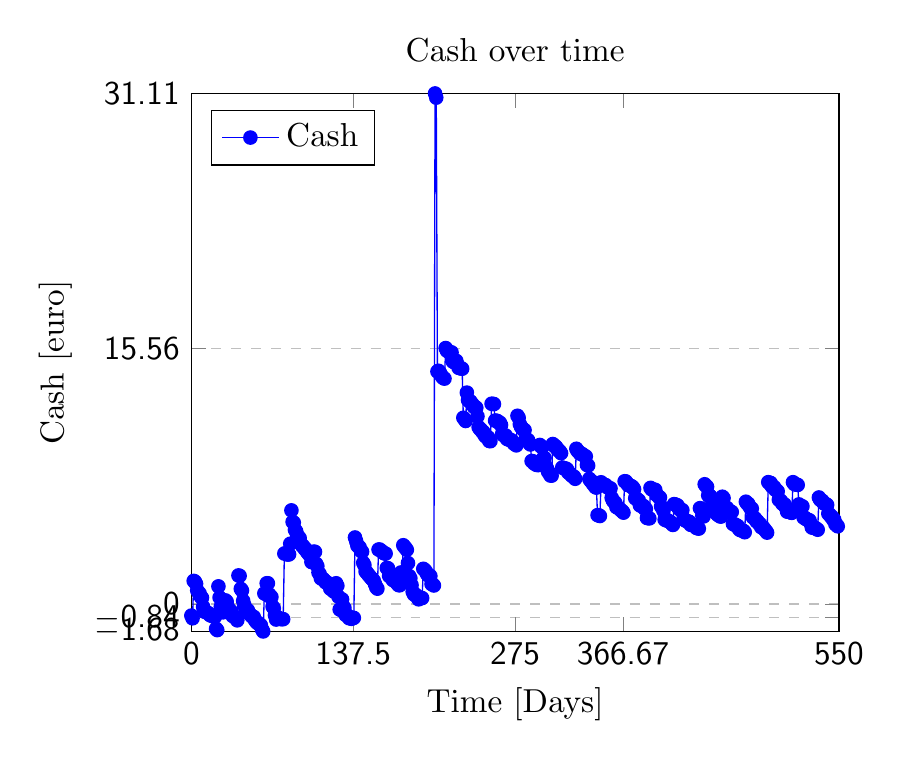
\begin{tikzpicture}[thick,scale=1.2]
\begin{axis}[
title={Cash over time},
xlabel={Time [Days]},
ylabel={Cash [euro]},
xmin=0,xmax=550,
ymin=-1.68,ymax=31.112,
xtick={0,137.5,275,366.666666666667,550},
ytick={-1.68,-0.84,0,15.556,31.112},
legend pos=north west,
ymajorgrids=true,
grid style=dashed,
]
\addplot[
color=blue,
mark=*,
]
coordinates {
(0,-0.713)(1,-0.878)(2,1.4)(3,1.36)(4,1.223)(5,0.822)(6,0.703)(7,0.636)(8,0.431)(9,0.37)(10,-0.183)(11,-0.469)(12,-0.487)(13,-0.512)(14,-0.547)(15,-0.617)(16,-0.695)(17,-0.715)(18,-0.729)(19,-0.772)(20,-0.792)(21,-1.515)(22,-1.599)(23,1.068)(24,0.388)(25,-0.181)(26,-0.339)(27,-0.515)(28,0.107)(29,0.212)(30,0.138)(31,-0.201)(32,-0.4)(33,-0.4)(34,-0.48)(35,-0.735)(36,-0.759)(37,-0.819)(38,-0.828)(39,-1.005)(40,1.734)(41,1.707)(42,0.916)(43,0.815)(44,0.187)(45,-0.071)(46,-0.325)(47,-0.361)(48,-0.384)(49,-0.595)(50,-0.639)(51,-0.739)(52,-0.794)(53,-0.794)(54,-0.988)(55,-1.084)(56,-1.164)(57,-1.189)(58,-1.239)(59,-1.299)(60,-1.553)(61,-1.68)(62,0.638)(63,0.605)(64,1.255)(65,1.255)(66,0.585)(67,0.424)(68,0.42)(69,-0.165)(70,-0.263)(71,-0.686)(72,-0.954)(73,-0.908)(74,-0.844)(75,-0.902)(76,-0.925)(77,-0.931)(78,-0.931)(79,3.069)(80,3.079)(81,3.025)(82,3.011)(83,3.016)(84,3.666)(85,5.7)(86,4.996)(87,4.947)(88,4.516)(89,4.428)(90,4.189)(91,4.069)(92,4.009)(93,3.684)(94,3.54)(95,3.52)(96,3.37)(97,3.35)(98,3.192)(99,3.112)(100,3.011)(101,2.947)(102,2.552)(103,2.537)(104,3.187)(105,3.171)(106,2.443)(107,2.297)(108,1.91)(109,1.815)(110,1.557)(111,1.541)(112,1.513)(113,1.417)(114,1.317)(115,1.317)(116,1.237)(117,1.133)(118,0.926)(119,0.914)(120,0.839)(121,0.753)(122,0.735)(123,1.256)(124,1.105)(125,0.435)(126,-0.34)(127,-0.368)(128,0.274)(129,-0.169)(130,-0.237)(131,-0.67)(132,-0.68)(133,-0.74)(134,-0.876)(135,-0.83)(136,-0.912)(137,-0.854)(138,-0.854)(139,4.046)(140,3.812)(141,3.547)(142,3.501)(143,3.44)(144,3.236)(145,3.175)(146,2.502)(147,2.358)(148,1.975)(149,1.913)(150,1.802)(151,1.726)(152,1.636)(153,1.546)(154,1.484)(155,1.404)(156,1.203)(157,1.014)(158,0.927)(159,3.312)(160,3.311)(161,3.246)(162,3.195)(163,3.115)(164,3.073)(165,3.064)(166,2.187)(167,2.171)(168,1.703)(169,1.673)(170,1.593)(171,1.461)(172,1.43)(173,1.425)(174,1.319)(175,1.226)(176,1.142)(177,1.134)(178,1.912)(179,1.902)(180,3.574)(181,3.474)(182,3.398)(183,3.292)(184,2.486)(185,1.697)(186,1.562)(187,1.147)(188,0.738)(189,0.58)(190,0.547)(191,0.529)(192,0.408)(193,0.277)(194,0.368)(195,0.353)(196,0.353)(197,2.137)(198,2.077)(199,2)(200,1.848)(201,1.747)(202,1.735)(203,1.699)(204,1.211)(205,1.193)(206,1.12)(207,31.112)(208,30.856)(209,14.164)(210,14.207)(211,14.097)(212,13.966)(213,13.837)(214,13.764)(215,13.73)(216,15.593)(217,15.433)(218,15.415)(219,15.345)(220,15.334)(221,15.329)(222,14.777)(223,14.732)(224,14.715)(225,14.814)(226,14.594)(227,14.39)(228,14.37)(229,14.353)(230,14.334)(231,11.343)(232,11.265)(233,11.148)(234,12.878)(235,12.428)(236,12.362)(237,12.342)(238,12.226)(239,12.147)(240,12.007)(241,12.002)(242,11.954)(243,11.433)(244,10.77)(245,10.665)(246,10.623)(247,10.493)(248,10.48)(249,10.285)(250,10.201)(251,10.163)(252,10.156)(253,9.929)(254,9.917)(255,12.199)(256,12.188)(257,12.18)(258,11.174)(259,11.159)(260,11.144)(261,11.052)(262,11.045)(263,10.902)(264,10.361)(265,10.277)(266,10.27)(267,10.259)(268,10.058)(269,10.029)(270,9.998)(271,9.99)(272,9.964)(273,9.875)(274,9.763)(275,9.752)(276,9.661)(277,11.465)(278,11.346)(279,10.954)(280,10.789)(281,10.714)(282,10.608)(283,10.592)(284,10.076)(285,10.004)(286,9.981)(287,9.796)(288,9.716)(289,8.705)(290,8.698)(291,8.564)(292,8.559)(293,8.472)(294,8.467)(295,8.463)(296,9.685)(297,9.59)(298,9.552)(299,8.899)(300,8.893)(301,8.362)(302,8.262)(303,8.049)(304,7.979)(305,7.824)(306,7.816)(307,9.743)(308,9.633)(309,9.623)(310,9.543)(311,9.402)(312,9.364)(313,9.291)(314,9.186)(315,8.309)(316,8.281)(317,8.255)(318,8.246)(319,8.21)(320,8.02)(321,7.965)(322,7.917)(323,7.817)(324,7.775)(325,7.751)(326,7.625)(327,9.455)(328,9.322)(329,9.276)(330,9.162)(331,9.158)(332,9.128)(333,9.064)(334,9.012)(335,8.988)(336,8.472)(337,8.429)(338,7.619)(339,7.506)(340,7.479)(341,7.316)(342,7.287)(343,7.126)(344,7.086)(345,5.41)(346,5.4)(347,5.356)(348,7.411)(349,7.285)(350,7.273)(351,7.248)(352,7.236)(353,7.13)(354,7.082)(355,7.05)(356,7.042)(357,6.468)(358,6.298)(359,6.223)(360,6.164)(361,5.899)(362,5.891)(363,5.831)(364,5.776)(365,5.694)(366,5.648)(367,5.56)(368,7.472)(369,7.464)(370,7.352)(371,7.237)(372,7.231)(373,7.187)(374,7.168)(375,7.108)(376,6.987)(377,6.438)(378,6.414)(379,6.338)(380,6.307)(381,6.003)(382,5.982)(383,5.974)(384,5.966)(385,5.797)(386,5.79)(387,5.237)(388,5.226)(389,5.21)(390,7.071)(391,6.973)(392,6.966)(393,6.959)(394,6.951)(395,6.652)(396,6.599)(397,6.509)(398,6.483)(399,5.943)(400,5.843)(401,5.67)(402,5.139)(403,5.097)(404,5.088)(405,5.076)(406,5.009)(407,4.983)(408,4.893)(409,4.811)(410,6.08)(411,6.057)(412,6.025)(413,5.995)(414,5.819)(415,5.745)(416,5.722)(417,5.715)(418,5.202)(419,5.102)(420,5.091)(421,5.024)(422,5.016)(423,5.002)(424,4.826)(425,4.805)(426,4.795)(427,4.782)(428,4.758)(429,4.627)(430,4.61)(431,4.587)(432,5.834)(433,5.794)(434,5.388)(435,5.329)(436,7.29)(437,7.2)(438,7.135)(439,6.616)(440,6.609)(441,6.541)(442,6.37)(443,5.948)(444,5.923)(445,5.584)(446,5.522)(447,5.433)(448,5.398)(449,5.33)(450,5.323)(451,6.532)(452,6.453)(453,5.904)(454,5.879)(455,5.84)(456,5.728)(457,5.62)(458,5.607)(459,5.6)(460,4.875)(461,4.838)(462,4.831)(463,4.754)(464,4.751)(465,4.575)(466,4.504)(467,4.482)(468,4.474)(469,4.451)(470,4.368)(471,6.226)(472,6.118)(473,6.1)(474,5.944)(475,5.824)(476,5.808)(477,5.27)(478,5.255)(479,5.186)(480,5.03)(481,5.023)(482,4.897)(483,4.867)(484,4.674)(485,4.65)(486,4.635)(487,4.528)(488,4.439)(489,4.342)(490,7.42)(491,7.36)(492,7.371)(493,7.162)(494,7.147)(495,7.114)(496,6.952)(497,6.927)(498,6.858)(499,6.349)(500,6.32)(501,6.252)(502,6.1)(503,6.074)(504,6.052)(505,5.87)(506,5.623)(507,5.615)(508,5.604)(509,5.575)(510,5.548)(511,7.417)(512,7.312)(513,7.29)(514,7.265)(515,7.252)(516,6.064)(517,5.958)(518,5.954)(519,5.943)(520,5.261)(521,5.253)(522,5.168)(523,5.144)(524,5.115)(525,5.093)(526,4.9)(527,4.655)(528,4.648)(529,4.639)(530,4.63)(531,4.565)(532,4.52)(533,6.485)(534,6.354)(535,6.305)(536,6.278)(537,6.141)(538,6.105)(539,6.078)(540,6.031)(541,5.502)(542,5.456)(543,5.334)(544,5.314)(545,5.144)(546,5.137)(547,4.855)(548,4.823)(549,4.728)
};
\legend{Cash}
\end{axis}
\end{tikzpicture}

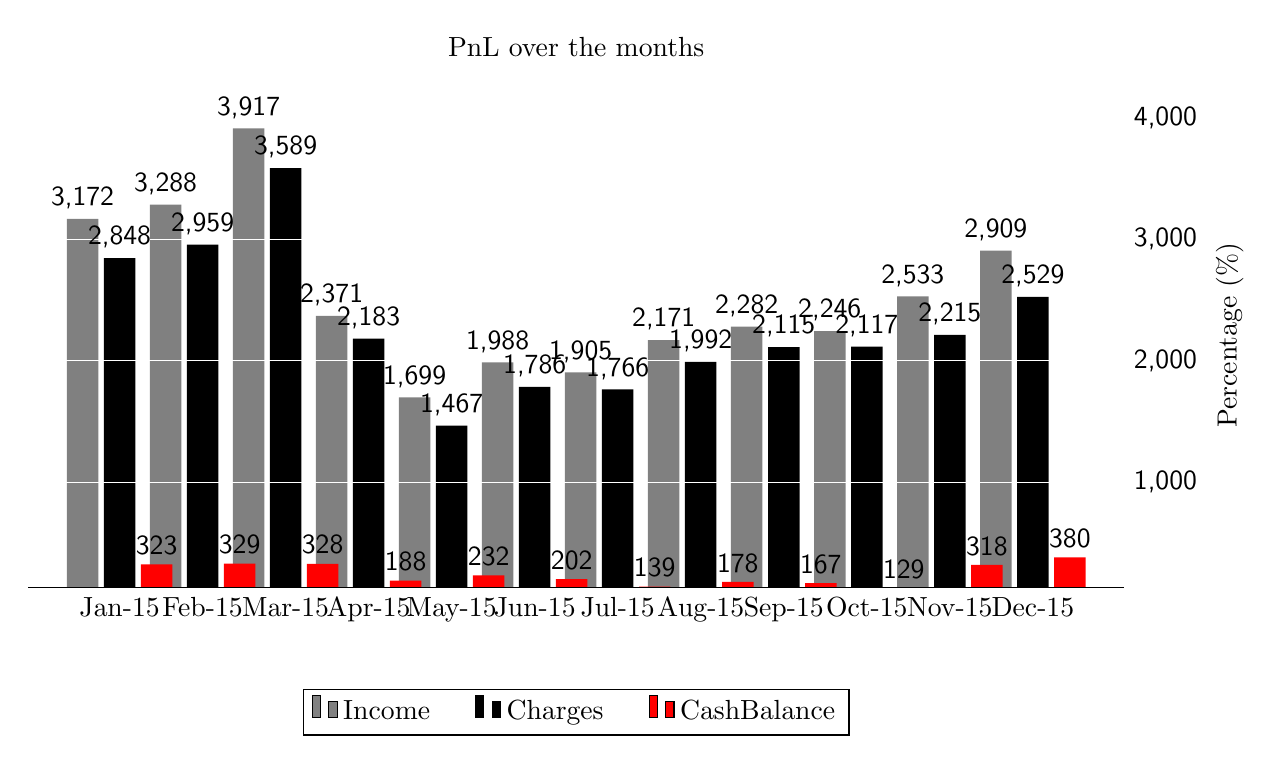
\begin{tikzpicture}[thick, scale=1]
\begin{axis}[
title={Kapital over time},
ybar, axis on top,
title={PnL over the months},
height=8cm, width=15.5cm,
bar width=0.4cm,
ymajorgrids, tick align=inside,
major grid style={draw=white},
enlarge y limits={value=.1,upper},
axis x line*=bottom,
axis y line*=right,
y axis line style={opacity=0},
tickwidth=0pt,
enlarge x limits=true,
legend style={
at={(0.5,-0.2)},
anchor=north,
legend columns=-1,
/tikz/every even column/.append style={column sep=0.5cm}
},
ylabel={Percentage (\%)},
symbolic x coords={
xlabel={Time [Days]},
ylabel={Kapital [euro]},
ymin=-4.956,ymax=27.836,
Jan-15,Feb-15,Mar-15,Apr-15,May-15,Jun-15,Jul-15,Aug-15,Sep-15,Oct-15,Nov-15,Dec-15},xtick=data,
nodes near coords={
\pgfmathprintnumber[precision=0]{\pgfplotspointmeta}
}
]
\addplot [draw=none, fill=black!50] coordinates {
(Jan-15,3171.67)
(Feb-15,3288.125)
(Mar-15,3916.859)
(Apr-15,2371.335)
(May-15,1699.039)
(Jun-15,1987.688)
(Jul-15,1904.966)
(Aug-15,2170.602)
(Sep-15,2281.823)
(Oct-15,2246.281)
(Nov-15,2533.229)
(Dec-15,2908.756)
};
\addplot [draw=none, fill=black!100] coordinates {
(Jan-15,2848.301)
(Feb-15,2958.914)
(Mar-15,3589.333)
(Apr-15,2183.188)
(May-15,1467.326)
(Jun-15,1785.85)
(Jul-15,1766.312)
(Aug-15,1992.222)
(Sep-15,2114.79)
(Oct-15,2117.486)
(Nov-15,2215.477)
(Dec-15,2528.859)
};
\addplot [draw=none, fill=red!100] coordinates {
(Jan-15,323.369)
(Feb-15,329.211)
(Mar-15,327.526)
(Apr-15,188.147)
(May-15,231.713)
(Jun-15,201.838)
(Jul-15,138.654)
(Aug-15,178.38)
(Sep-15,167.033)
(Oct-15,128.795)
(Nov-15,317.752)
(Dec-15,379.897)
};

\legend{Income,Charges,CashBalance}
\end{axis}
\end{tikzpicture}


\subsubsection{Worst cashflows}
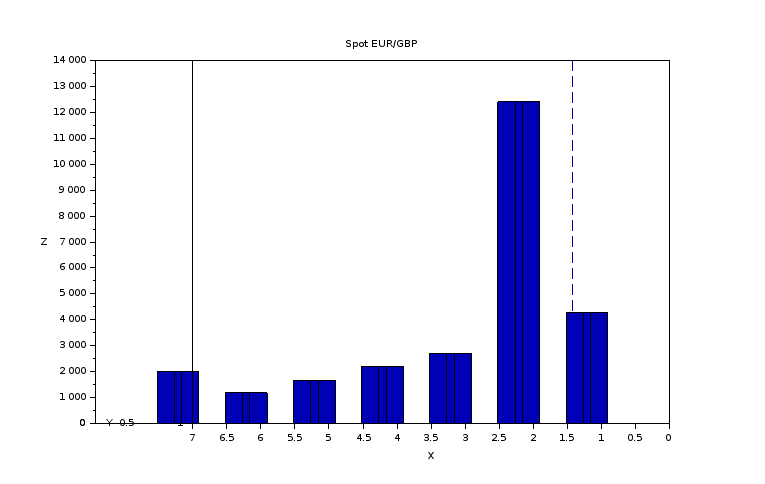
\includegraphics[scale=0.6]{Vector.png}

This where science enter the game as here can call scilab and there is no limit at what we could calculate... fascinating!
How do we populate Scilab with Negative numbers where there are Debits and Positive numbers for the Credit
\subsubsection{Cashbalance with a moving average}
\includegraphics[scale=0.6]{../Maths/Scilab-cashBalance.png}

\subsubsection{Map Of The Charges}
%\includepdf[pages={1}]{MapOfTheCharges.pdf}
\input{MapOfTheCharges}
\subsubsection{Monthly Charges}
\includegraphics[scale=0.6]{resize_charges.png}
\includegraphics[scale=0.6]{../Maths/Scilab-categories.png}

%\subsubsection{Cash curve}
%Funny cashflow/kapital superior to percent\\
%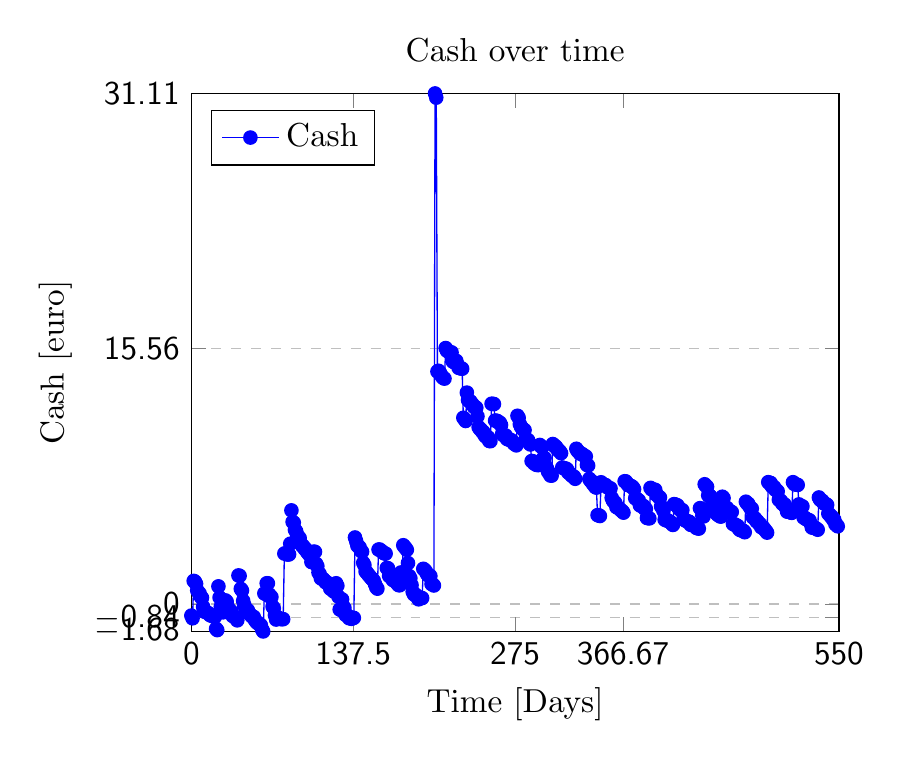
\begin{tikzpicture}[thick,scale=1.2]
\begin{axis}[
title={Cash over time},
xlabel={Time [Days]},
ylabel={Cash [euro]},
xmin=0,xmax=550,
ymin=-1.68,ymax=31.112,
xtick={0,137.5,275,366.666666666667,550},
ytick={-1.68,-0.84,0,15.556,31.112},
legend pos=north west,
ymajorgrids=true,
grid style=dashed,
]
\addplot[
color=blue,
mark=*,
]
coordinates {
(0,-0.713)(1,-0.878)(2,1.4)(3,1.36)(4,1.223)(5,0.822)(6,0.703)(7,0.636)(8,0.431)(9,0.37)(10,-0.183)(11,-0.469)(12,-0.487)(13,-0.512)(14,-0.547)(15,-0.617)(16,-0.695)(17,-0.715)(18,-0.729)(19,-0.772)(20,-0.792)(21,-1.515)(22,-1.599)(23,1.068)(24,0.388)(25,-0.181)(26,-0.339)(27,-0.515)(28,0.107)(29,0.212)(30,0.138)(31,-0.201)(32,-0.4)(33,-0.4)(34,-0.48)(35,-0.735)(36,-0.759)(37,-0.819)(38,-0.828)(39,-1.005)(40,1.734)(41,1.707)(42,0.916)(43,0.815)(44,0.187)(45,-0.071)(46,-0.325)(47,-0.361)(48,-0.384)(49,-0.595)(50,-0.639)(51,-0.739)(52,-0.794)(53,-0.794)(54,-0.988)(55,-1.084)(56,-1.164)(57,-1.189)(58,-1.239)(59,-1.299)(60,-1.553)(61,-1.68)(62,0.638)(63,0.605)(64,1.255)(65,1.255)(66,0.585)(67,0.424)(68,0.42)(69,-0.165)(70,-0.263)(71,-0.686)(72,-0.954)(73,-0.908)(74,-0.844)(75,-0.902)(76,-0.925)(77,-0.931)(78,-0.931)(79,3.069)(80,3.079)(81,3.025)(82,3.011)(83,3.016)(84,3.666)(85,5.7)(86,4.996)(87,4.947)(88,4.516)(89,4.428)(90,4.189)(91,4.069)(92,4.009)(93,3.684)(94,3.54)(95,3.52)(96,3.37)(97,3.35)(98,3.192)(99,3.112)(100,3.011)(101,2.947)(102,2.552)(103,2.537)(104,3.187)(105,3.171)(106,2.443)(107,2.297)(108,1.91)(109,1.815)(110,1.557)(111,1.541)(112,1.513)(113,1.417)(114,1.317)(115,1.317)(116,1.237)(117,1.133)(118,0.926)(119,0.914)(120,0.839)(121,0.753)(122,0.735)(123,1.256)(124,1.105)(125,0.435)(126,-0.34)(127,-0.368)(128,0.274)(129,-0.169)(130,-0.237)(131,-0.67)(132,-0.68)(133,-0.74)(134,-0.876)(135,-0.83)(136,-0.912)(137,-0.854)(138,-0.854)(139,4.046)(140,3.812)(141,3.547)(142,3.501)(143,3.44)(144,3.236)(145,3.175)(146,2.502)(147,2.358)(148,1.975)(149,1.913)(150,1.802)(151,1.726)(152,1.636)(153,1.546)(154,1.484)(155,1.404)(156,1.203)(157,1.014)(158,0.927)(159,3.312)(160,3.311)(161,3.246)(162,3.195)(163,3.115)(164,3.073)(165,3.064)(166,2.187)(167,2.171)(168,1.703)(169,1.673)(170,1.593)(171,1.461)(172,1.43)(173,1.425)(174,1.319)(175,1.226)(176,1.142)(177,1.134)(178,1.912)(179,1.902)(180,3.574)(181,3.474)(182,3.398)(183,3.292)(184,2.486)(185,1.697)(186,1.562)(187,1.147)(188,0.738)(189,0.58)(190,0.547)(191,0.529)(192,0.408)(193,0.277)(194,0.368)(195,0.353)(196,0.353)(197,2.137)(198,2.077)(199,2)(200,1.848)(201,1.747)(202,1.735)(203,1.699)(204,1.211)(205,1.193)(206,1.12)(207,31.112)(208,30.856)(209,14.164)(210,14.207)(211,14.097)(212,13.966)(213,13.837)(214,13.764)(215,13.73)(216,15.593)(217,15.433)(218,15.415)(219,15.345)(220,15.334)(221,15.329)(222,14.777)(223,14.732)(224,14.715)(225,14.814)(226,14.594)(227,14.39)(228,14.37)(229,14.353)(230,14.334)(231,11.343)(232,11.265)(233,11.148)(234,12.878)(235,12.428)(236,12.362)(237,12.342)(238,12.226)(239,12.147)(240,12.007)(241,12.002)(242,11.954)(243,11.433)(244,10.77)(245,10.665)(246,10.623)(247,10.493)(248,10.48)(249,10.285)(250,10.201)(251,10.163)(252,10.156)(253,9.929)(254,9.917)(255,12.199)(256,12.188)(257,12.18)(258,11.174)(259,11.159)(260,11.144)(261,11.052)(262,11.045)(263,10.902)(264,10.361)(265,10.277)(266,10.27)(267,10.259)(268,10.058)(269,10.029)(270,9.998)(271,9.99)(272,9.964)(273,9.875)(274,9.763)(275,9.752)(276,9.661)(277,11.465)(278,11.346)(279,10.954)(280,10.789)(281,10.714)(282,10.608)(283,10.592)(284,10.076)(285,10.004)(286,9.981)(287,9.796)(288,9.716)(289,8.705)(290,8.698)(291,8.564)(292,8.559)(293,8.472)(294,8.467)(295,8.463)(296,9.685)(297,9.59)(298,9.552)(299,8.899)(300,8.893)(301,8.362)(302,8.262)(303,8.049)(304,7.979)(305,7.824)(306,7.816)(307,9.743)(308,9.633)(309,9.623)(310,9.543)(311,9.402)(312,9.364)(313,9.291)(314,9.186)(315,8.309)(316,8.281)(317,8.255)(318,8.246)(319,8.21)(320,8.02)(321,7.965)(322,7.917)(323,7.817)(324,7.775)(325,7.751)(326,7.625)(327,9.455)(328,9.322)(329,9.276)(330,9.162)(331,9.158)(332,9.128)(333,9.064)(334,9.012)(335,8.988)(336,8.472)(337,8.429)(338,7.619)(339,7.506)(340,7.479)(341,7.316)(342,7.287)(343,7.126)(344,7.086)(345,5.41)(346,5.4)(347,5.356)(348,7.411)(349,7.285)(350,7.273)(351,7.248)(352,7.236)(353,7.13)(354,7.082)(355,7.05)(356,7.042)(357,6.468)(358,6.298)(359,6.223)(360,6.164)(361,5.899)(362,5.891)(363,5.831)(364,5.776)(365,5.694)(366,5.648)(367,5.56)(368,7.472)(369,7.464)(370,7.352)(371,7.237)(372,7.231)(373,7.187)(374,7.168)(375,7.108)(376,6.987)(377,6.438)(378,6.414)(379,6.338)(380,6.307)(381,6.003)(382,5.982)(383,5.974)(384,5.966)(385,5.797)(386,5.79)(387,5.237)(388,5.226)(389,5.21)(390,7.071)(391,6.973)(392,6.966)(393,6.959)(394,6.951)(395,6.652)(396,6.599)(397,6.509)(398,6.483)(399,5.943)(400,5.843)(401,5.67)(402,5.139)(403,5.097)(404,5.088)(405,5.076)(406,5.009)(407,4.983)(408,4.893)(409,4.811)(410,6.08)(411,6.057)(412,6.025)(413,5.995)(414,5.819)(415,5.745)(416,5.722)(417,5.715)(418,5.202)(419,5.102)(420,5.091)(421,5.024)(422,5.016)(423,5.002)(424,4.826)(425,4.805)(426,4.795)(427,4.782)(428,4.758)(429,4.627)(430,4.61)(431,4.587)(432,5.834)(433,5.794)(434,5.388)(435,5.329)(436,7.29)(437,7.2)(438,7.135)(439,6.616)(440,6.609)(441,6.541)(442,6.37)(443,5.948)(444,5.923)(445,5.584)(446,5.522)(447,5.433)(448,5.398)(449,5.33)(450,5.323)(451,6.532)(452,6.453)(453,5.904)(454,5.879)(455,5.84)(456,5.728)(457,5.62)(458,5.607)(459,5.6)(460,4.875)(461,4.838)(462,4.831)(463,4.754)(464,4.751)(465,4.575)(466,4.504)(467,4.482)(468,4.474)(469,4.451)(470,4.368)(471,6.226)(472,6.118)(473,6.1)(474,5.944)(475,5.824)(476,5.808)(477,5.27)(478,5.255)(479,5.186)(480,5.03)(481,5.023)(482,4.897)(483,4.867)(484,4.674)(485,4.65)(486,4.635)(487,4.528)(488,4.439)(489,4.342)(490,7.42)(491,7.36)(492,7.371)(493,7.162)(494,7.147)(495,7.114)(496,6.952)(497,6.927)(498,6.858)(499,6.349)(500,6.32)(501,6.252)(502,6.1)(503,6.074)(504,6.052)(505,5.87)(506,5.623)(507,5.615)(508,5.604)(509,5.575)(510,5.548)(511,7.417)(512,7.312)(513,7.29)(514,7.265)(515,7.252)(516,6.064)(517,5.958)(518,5.954)(519,5.943)(520,5.261)(521,5.253)(522,5.168)(523,5.144)(524,5.115)(525,5.093)(526,4.9)(527,4.655)(528,4.648)(529,4.639)(530,4.63)(531,4.565)(532,4.52)(533,6.485)(534,6.354)(535,6.305)(536,6.278)(537,6.141)(538,6.105)(539,6.078)(540,6.031)(541,5.502)(542,5.456)(543,5.334)(544,5.314)(545,5.144)(546,5.137)(547,4.855)(548,4.823)(549,4.728)
};
\legend{Cash}
\end{axis}
\end{tikzpicture}

%Checklists.tex:%\includegraphics[scale=0.5]{stockchart.pdf}}

%\subsubsection{Cash curve from Scilab man!}
%\includegraphics[scale=0.6]{Scilab-cashBalance.png}

\subsubsection{Uncategorized Cashflows}
%\begin{longtable}{|c|c|c|c|c|}
\hline
\multicolumn{5}{|c|}{Cashflows} \\
\hline
Date & Income & Charges & PnL & NumDays\\
\hline
2021-01-13 & 96890 & 92162 & 4728 & 7531\\
\hline
2017-04-20 & 96890 & 92162 & 4728 & 6167\\
\hline
2017-04-19 & 96890 & 92067 & 4823 & 6166\\
\hline
2017-04-18 & 96890 & 92035 & 4855 & 6165\\
\hline
2017-04-14 & 96890 & 91753 & 5137 & 6161\\
\hline
2017-04-13 & 96890 & 91746 & 5144 & 6160\\
\hline
2017-04-12 & 96890 & 91576 & 5314 & 6159\\
\hline
2017-04-11 & 96890 & 91556 & 5334 & 6158\\
\hline
2017-04-10 & 96890 & 91434 & 5456 & 6157\\
\hline
2017-04-07 & 96890 & 91388 & 5502 & 6154\\
\hline
2017-04-06 & 96890 & 90859 & 6031 & 6153\\
\hline
2017-04-05 & 96890 & 90812 & 6078 & 6152\\
\hline
2017-04-04 & 96890 & 90785 & 6105 & 6151\\
\hline
2017-04-03 & 96890 & 90749 & 6141 & 6150\\
\hline
2017-03-31 & 96890 & 90612 & 6278 & 6147\\
\hline
 ... & ... & ... & ... & ... & ...\\
\hline
 Total &  &  &  &  & \\
\hline
\end{longtable}

\begin{longtable}{|c|c|c|c|}
\hline
\multicolumn{4}{|c|}{Cashflows} \\
\hline
Category & Libelle & Debit \\
\hline
Other & CAP300BOWLINGTADEN14/01 & 21\\
\hline
Other & OSCAROPARIS07/01 & 104\\
\hline
Other & BBNDINAN10/11 & 70\\
\hline
Other & LYVETDISTRIBUTIONLAVICO09/11 & 9\\
\hline
Other & DIFERTIDINAN30/10 & 59\\
\hline
Other & 2888432 & 30\\
\hline
Other & 2888433 & 57\\
\hline
Other & MAMBIHANLANVALLAY19/08 & 7\\
\hline
Other & HUITAHUITPLOUBALAY21/06 & 5\\
\hline
Other & LAPAILLOTTEPAIMPOL08/05 & 8\\
\hline
Other & 5216299 & 153\\
\hline
Other & FNACDIRECTIVRYSURSEINE12/08 & 50\\
\hline
Other & 5216298 & 23\\
\hline
Other & MUSEESTEMARIE15/06 & 16\\
\hline
Other & LANDIDISTRIBUT13/06 & 8\\
\hline
Other & RESTOCECCODINAN27/05 & 18\\
\hline
Other & MUZIKANAODINAN18/05 & 18\\
\hline
Other & 5216296 & 4\\
\hline
Other & 5216297 & 21\\
\hline
Other & 5216294 & 71\\
\hline
\end{longtable}

\subsubsection{Cashflows of the last 31 days}
\begin{longtable}{|c|c|c|c|c|}
\hline
\multicolumn{5}{|c|}{Cashflows} \\
\hline
Date & Category & Libelle & Debit & \\
\hline
2018-12-31 00:00:00 & Food & CARREFOURCITYDINAN30/12 & 12 & \\
\hline
2018-12-31 00:00:00 & Toxics & LEHAVANEDINAN30/12 & 17 & \\
\hline
2018-12-31 00:00:00 & Food & MOKODINAN28/12 & 21 & \\
\hline
2018-12-31 00:00:00 & Toxics & SNCBUSNEL-HERVDINAN28/12 & 16 & \\
\hline
2018-12-31 00:00:00 & Food & INTERMARCHETADEN28/12 & 19 & \\
\hline
2018-12-28 00:00:00 & Bank & FraisIrreg.EtIncidents11/2018 & 80 & \\
\hline
2018-12-28 00:00:00 & Food & INTERMARCHETADEN27/12 & 14 & \\
\hline
2018-12-28 00:00:00 & Toxics & SNCBUSNEL-HERVDINAN27/12 & 16 & \\
\hline
2018-12-28 00:00:00 & Other & 3233246 & 474 & \\
\hline
2018-12-27 00:00:00 & Toxics & LECARILLONDINAN23/12 & 16 & \\
\hline
2018-12-27 00:00:00 & Food & INTERMARCHENFCTADEN26/12 & 6 & \\
\hline
2018-12-26 00:00:00 & Food & SOMOBADACTADEN24/12 & 25 & \\
\hline
2018-12-26 00:00:00 & Toxics & SNCBUSNEL-HERVDINAN24/12 & 24 & \\
\hline
2018-12-26 00:00:00 & Food & INTERMARCHETADEN24/12 & 19 & \\
\hline
2018-12-26 00:00:00 & Food & INTERMARCHENFCTADEN24/12 & 3 & \\
\hline
2018-12-24 00:00:00 & Cash & LCLDINAN23/1216H24 & 60 & \\
\hline
2018-12-24 00:00:00 & Toxics & BARVEDETTESDINAN21/12 & 17 & \\
\hline
2018-12-24 00:00:00 & Food & INTERMARCHENFCTADEN21/12 & 8 & \\
\hline
2018-12-24 00:00:00 & Toxics & LORANGEBLEUEQUEVERT21/12 & 418 & \\
\hline
2018-12-24 00:00:00 & Toxics & BARDESVEDETTEDINAN23/12 & 29 & \\
\hline
2018-12-24 00:00:00 & Food & INTERMARCHETADEN22/12 & 15 & \\
\hline
2018-12-24 00:00:00 & Toxics & MONDEMERVEILLEUXDINAN23/12 & 25 & \\
\hline
2018-12-24 00:00:00 & Other & BISCUITERDUGRAALDINAN23/12 & 59 & \\
\hline
2018-12-24 00:00:00 & Toxics & SNCBUSNEL-HERVDINAN22/12 & 16 & \\
\hline
2018-12-21 00:00:00 & Toxics & BARDESVEDETTEDINAN20/12 & 47 & \\
\hline
2018-12-20 00:00:00 & Food & INTERMARCHENFCTADEN19/12 & 7 & \\
\hline
2018-12-19 00:00:00 & Debt & CRCAMDUFINISTERE & 185 & \\
\hline
2018-12-19 00:00:00 & Toxics & SNCBUSNEL-HERVDINAN18/12 & 16 & \\
\hline
2018-12-19 00:00:00 & Food & SOMOBADACTADEN18/12 & 57 & \\
\hline
2018-12-18 00:00:00 & Food & INTERMARCHENFCTADEN17/12 & 5 & \\
\hline
2018-12-18 00:00:00 & Toxics & SNCBUSNEL-HERVDINAN17/12 & 16 & \\
\hline
2018-12-17 00:00:00 & Cash & DINANINTERMARCH16/1212H28 & 60 & \\
\hline
2018-12-17 00:00:00 & Other & RESTOCECCODINAN14/12 & 4 & \\
\hline
2018-12-17 00:00:00 & Food & INTERMARCHENFCTADEN16/12 & 8 & \\
\hline
2018-12-17 00:00:00 & Food & INTERMARCHETADEN15/12 & 23 & \\
\hline
2018-12-17 00:00:00 & Food & INTERMARCHENFCTADEN14/12 & 8 & \\
\hline
2018-12-17 00:00:00 & Toxics & SNCBUSNEL-HERVDINAN15/12 & 16 & \\
\hline
2018-12-17 00:00:00 & Telephone & SFR & 43 & \\
\hline
2018-12-14 00:00:00 & Food & SOMOBADACTADEN13/12 & 27 & \\
\hline
2018-12-14 00:00:00 & Food & INTERMARCHENFCTADEN13/12 & 7 & \\
\hline
2018-12-14 00:00:00 & Toxics & SNCBUSNEL-HERVDINAN13/12 & 17 & \\
\hline
2018-12-13 00:00:00 & Other & Action4185Dinan-Queve12/12 & 5 & \\
\hline
2018-12-13 00:00:00 & Other & CHEZLUDODINAN12/12 & 24 & \\
\hline
2018-12-12 00:00:00 & Food & INTERMARCHENFCTADEN11/12 & 5 & \\
\hline
2018-12-11 00:00:00 & Food & INTERMARCHETADEN10/12 & 21 & \\
\hline
2018-12-11 00:00:00 & Toxics & SNCBUSNEL-HERVDINAN10/12 & 16 & \\
\hline
2018-12-10 00:00:00 & Food & SOMOBADACTADEN09/12 & 7 & \\
\hline
2018-12-10 00:00:00 & Toxics & BARDESVEDETTEDINAN08/12 & 14 & \\
\hline
2018-12-10 00:00:00 & Food & INTERMARCHETADEN07/12 & 6 & \\
\hline
2018-12-10 00:00:00 & Other & LABRICKROUGEDINAN07/12 & 20 & \\
\hline
2018-12-10 00:00:00 & Food & CHEZBONGRAINDINAN07/12 & 65 & \\
\hline
2018-12-10 00:00:00 & Toxics & BARDESVEDETTEDINAN09/12 & 18 & \\
\hline
2018-12-10 00:00:00 & Food & LATYPICDINAN08/12 & 28 & \\
\hline
2018-12-10 00:00:00 & Toxics & AUVIEUXSTSAUVEURDINAN08/12 & 10 & \\
\hline
2018-12-10 00:00:00 & Toxics & LEGAULOISDINAN08/12 & 16 & \\
\hline
2018-12-10 00:00:00 & Debt & CRCAMDUFINISTERE & 509 & \\
\hline
2018-12-07 00:00:00 & Toxics & SNCBUSNEL-HERVDINAN06/12 & 24 & \\
\hline
2018-12-07 00:00:00 & Food & INTERMARCHENFCTADEN06/12 & 5 & \\
\hline
 ... & ... & ... & ... & \\
\hline
 Total & 144153.00011040078 & 147437.00011040078 & 3284 & \\
\hline
\end{longtable}

%\begin{bchart}[min=0,max=11366,step=3788,unit=k\texteuro]
\bcbar[label=Other]{2}\\
\smallskip
\bcbar[label=Other]{10}\\
\smallskip
\bcbar[label=Other]{7}\\
\smallskip
\bcbar[label=Other]{0}\\
\smallskip
\bcbar[label=Other]{5}\\
\smallskip
\bcbar[label=Other]{3}\\
\smallskip
\bcbar[label=Other]{5}\\
\smallskip
\bcbar[label=Other]{0}\\
\smallskip
\bcbar[label=Other]{0}\\
\smallskip
\bcbar[label=Other]{0}\\
\smallskip
\bcbar[label=Other]{15}\\
\smallskip
\bcbar[label=Other]{5}\\
\smallskip
\bcbar[label=Other]{2}\\
\smallskip
\bcbar[label=Other]{1}\\
\smallskip
\bcbar[label=Other]{0}\\
\smallskip
\bcbar[label=Other]{1}\\
\smallskip
\bcbar[label=Other]{1}\\
\smallskip
\bcbar[label=Other]{0}\\
\smallskip
\bcbar[label=Other]{2}\\
\smallskip
\bcbar[label=Other]{7}\\
\smallskip
\end{bchart}

To be able to have data for the drift, you need to build a C++ insert like for the kapital
go through the dates in the cashflows, and calculate a drift based on this (modulo the salary) 
\subsubsection{Graph}
%\includegraphics[width=.8\textwidth]{PnL.png}
%\begin{bchart}[min=0,max=96,step=32,unit=k\texteuro]
\bcbar[label=Income]{96}\\
\smallskip
\bcbar[label=Charges]{92}\\
\smallskip
\bcbar[label=Drift]{4}\\
\smallskip
\bcbar[label=Income]{96}\\
\smallskip
\bcbar[label=Charges]{92}\\
\smallskip
\bcbar[label=Drift]{4}\\
\smallskip
\bcbar[label=Income]{96}\\
\smallskip
\bcbar[label=Charges]{92}\\
\smallskip
\bcbar[label=Drift]{4}\\
\smallskip
\bcbar[label=Income]{96}\\
\smallskip
\bcbar[label=Charges]{92}\\
\smallskip
\bcbar[label=Drift]{4}\\
\smallskip
\bcbar[label=Income]{96}\\
\smallskip
\bcbar[label=Charges]{91}\\
\smallskip
\bcbar[label=Drift]{5}\\
\smallskip
\bcbar[label=Income]{96}\\
\smallskip
\bcbar[label=Charges]{91}\\
\smallskip
\bcbar[label=Drift]{5}\\
\smallskip
\bcbar[label=Income]{96}\\
\smallskip
\bcbar[label=Charges]{91}\\
\smallskip
\bcbar[label=Drift]{5}\\
\smallskip
\bcbar[label=Income]{96}\\
\smallskip
\bcbar[label=Charges]{91}\\
\smallskip
\bcbar[label=Drift]{5}\\
\smallskip
\bcbar[label=Income]{96}\\
\smallskip
\bcbar[label=Charges]{91}\\
\smallskip
\bcbar[label=Drift]{5}\\
\smallskip
\bcbar[label=Income]{96}\\
\smallskip
\bcbar[label=Charges]{91}\\
\smallskip
\bcbar[label=Drift]{5}\\
\smallskip
\bcbar[label=Income]{96}\\
\smallskip
\bcbar[label=Charges]{90}\\
\smallskip
\bcbar[label=Drift]{6}\\
\smallskip
\bcbar[label=Income]{96}\\
\smallskip
\bcbar[label=Charges]{90}\\
\smallskip
\bcbar[label=Drift]{6}\\
\smallskip
\bcbar[label=Income]{96}\\
\smallskip
\bcbar[label=Charges]{90}\\
\smallskip
\bcbar[label=Drift]{6}\\
\smallskip
\bcbar[label=Income]{96}\\
\smallskip
\bcbar[label=Charges]{90}\\
\smallskip
\bcbar[label=Drift]{6}\\
\smallskip
\bcbar[label=Income]{96}\\
\smallskip
\bcbar[label=Charges]{90}\\
\smallskip
\bcbar[label=Drift]{6}\\
\smallskip
\end{bchart}

%\input{Plot}
%Here we plot the cashflows over a certain limit. This should be moved to a histogramm for a better readability
%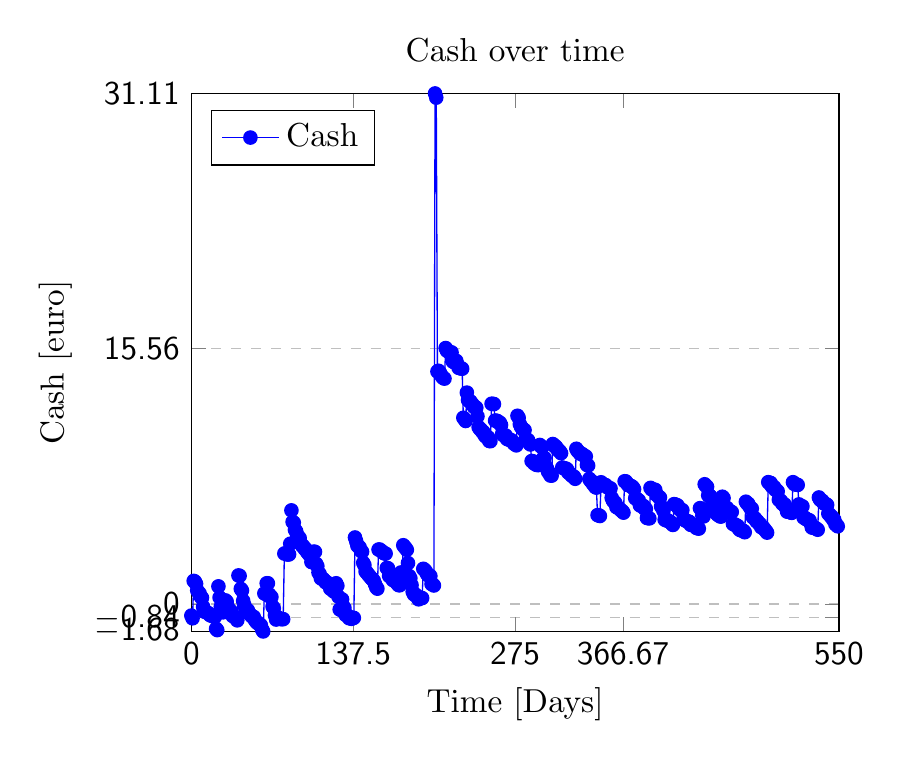
\begin{tikzpicture}[thick,scale=1.2]
\begin{axis}[
title={Cash over time},
xlabel={Time [Days]},
ylabel={Cash [euro]},
xmin=0,xmax=550,
ymin=-1.68,ymax=31.112,
xtick={0,137.5,275,366.666666666667,550},
ytick={-1.68,-0.84,0,15.556,31.112},
legend pos=north west,
ymajorgrids=true,
grid style=dashed,
]
\addplot[
color=blue,
mark=*,
]
coordinates {
(0,-0.713)(1,-0.878)(2,1.4)(3,1.36)(4,1.223)(5,0.822)(6,0.703)(7,0.636)(8,0.431)(9,0.37)(10,-0.183)(11,-0.469)(12,-0.487)(13,-0.512)(14,-0.547)(15,-0.617)(16,-0.695)(17,-0.715)(18,-0.729)(19,-0.772)(20,-0.792)(21,-1.515)(22,-1.599)(23,1.068)(24,0.388)(25,-0.181)(26,-0.339)(27,-0.515)(28,0.107)(29,0.212)(30,0.138)(31,-0.201)(32,-0.4)(33,-0.4)(34,-0.48)(35,-0.735)(36,-0.759)(37,-0.819)(38,-0.828)(39,-1.005)(40,1.734)(41,1.707)(42,0.916)(43,0.815)(44,0.187)(45,-0.071)(46,-0.325)(47,-0.361)(48,-0.384)(49,-0.595)(50,-0.639)(51,-0.739)(52,-0.794)(53,-0.794)(54,-0.988)(55,-1.084)(56,-1.164)(57,-1.189)(58,-1.239)(59,-1.299)(60,-1.553)(61,-1.68)(62,0.638)(63,0.605)(64,1.255)(65,1.255)(66,0.585)(67,0.424)(68,0.42)(69,-0.165)(70,-0.263)(71,-0.686)(72,-0.954)(73,-0.908)(74,-0.844)(75,-0.902)(76,-0.925)(77,-0.931)(78,-0.931)(79,3.069)(80,3.079)(81,3.025)(82,3.011)(83,3.016)(84,3.666)(85,5.7)(86,4.996)(87,4.947)(88,4.516)(89,4.428)(90,4.189)(91,4.069)(92,4.009)(93,3.684)(94,3.54)(95,3.52)(96,3.37)(97,3.35)(98,3.192)(99,3.112)(100,3.011)(101,2.947)(102,2.552)(103,2.537)(104,3.187)(105,3.171)(106,2.443)(107,2.297)(108,1.91)(109,1.815)(110,1.557)(111,1.541)(112,1.513)(113,1.417)(114,1.317)(115,1.317)(116,1.237)(117,1.133)(118,0.926)(119,0.914)(120,0.839)(121,0.753)(122,0.735)(123,1.256)(124,1.105)(125,0.435)(126,-0.34)(127,-0.368)(128,0.274)(129,-0.169)(130,-0.237)(131,-0.67)(132,-0.68)(133,-0.74)(134,-0.876)(135,-0.83)(136,-0.912)(137,-0.854)(138,-0.854)(139,4.046)(140,3.812)(141,3.547)(142,3.501)(143,3.44)(144,3.236)(145,3.175)(146,2.502)(147,2.358)(148,1.975)(149,1.913)(150,1.802)(151,1.726)(152,1.636)(153,1.546)(154,1.484)(155,1.404)(156,1.203)(157,1.014)(158,0.927)(159,3.312)(160,3.311)(161,3.246)(162,3.195)(163,3.115)(164,3.073)(165,3.064)(166,2.187)(167,2.171)(168,1.703)(169,1.673)(170,1.593)(171,1.461)(172,1.43)(173,1.425)(174,1.319)(175,1.226)(176,1.142)(177,1.134)(178,1.912)(179,1.902)(180,3.574)(181,3.474)(182,3.398)(183,3.292)(184,2.486)(185,1.697)(186,1.562)(187,1.147)(188,0.738)(189,0.58)(190,0.547)(191,0.529)(192,0.408)(193,0.277)(194,0.368)(195,0.353)(196,0.353)(197,2.137)(198,2.077)(199,2)(200,1.848)(201,1.747)(202,1.735)(203,1.699)(204,1.211)(205,1.193)(206,1.12)(207,31.112)(208,30.856)(209,14.164)(210,14.207)(211,14.097)(212,13.966)(213,13.837)(214,13.764)(215,13.73)(216,15.593)(217,15.433)(218,15.415)(219,15.345)(220,15.334)(221,15.329)(222,14.777)(223,14.732)(224,14.715)(225,14.814)(226,14.594)(227,14.39)(228,14.37)(229,14.353)(230,14.334)(231,11.343)(232,11.265)(233,11.148)(234,12.878)(235,12.428)(236,12.362)(237,12.342)(238,12.226)(239,12.147)(240,12.007)(241,12.002)(242,11.954)(243,11.433)(244,10.77)(245,10.665)(246,10.623)(247,10.493)(248,10.48)(249,10.285)(250,10.201)(251,10.163)(252,10.156)(253,9.929)(254,9.917)(255,12.199)(256,12.188)(257,12.18)(258,11.174)(259,11.159)(260,11.144)(261,11.052)(262,11.045)(263,10.902)(264,10.361)(265,10.277)(266,10.27)(267,10.259)(268,10.058)(269,10.029)(270,9.998)(271,9.99)(272,9.964)(273,9.875)(274,9.763)(275,9.752)(276,9.661)(277,11.465)(278,11.346)(279,10.954)(280,10.789)(281,10.714)(282,10.608)(283,10.592)(284,10.076)(285,10.004)(286,9.981)(287,9.796)(288,9.716)(289,8.705)(290,8.698)(291,8.564)(292,8.559)(293,8.472)(294,8.467)(295,8.463)(296,9.685)(297,9.59)(298,9.552)(299,8.899)(300,8.893)(301,8.362)(302,8.262)(303,8.049)(304,7.979)(305,7.824)(306,7.816)(307,9.743)(308,9.633)(309,9.623)(310,9.543)(311,9.402)(312,9.364)(313,9.291)(314,9.186)(315,8.309)(316,8.281)(317,8.255)(318,8.246)(319,8.21)(320,8.02)(321,7.965)(322,7.917)(323,7.817)(324,7.775)(325,7.751)(326,7.625)(327,9.455)(328,9.322)(329,9.276)(330,9.162)(331,9.158)(332,9.128)(333,9.064)(334,9.012)(335,8.988)(336,8.472)(337,8.429)(338,7.619)(339,7.506)(340,7.479)(341,7.316)(342,7.287)(343,7.126)(344,7.086)(345,5.41)(346,5.4)(347,5.356)(348,7.411)(349,7.285)(350,7.273)(351,7.248)(352,7.236)(353,7.13)(354,7.082)(355,7.05)(356,7.042)(357,6.468)(358,6.298)(359,6.223)(360,6.164)(361,5.899)(362,5.891)(363,5.831)(364,5.776)(365,5.694)(366,5.648)(367,5.56)(368,7.472)(369,7.464)(370,7.352)(371,7.237)(372,7.231)(373,7.187)(374,7.168)(375,7.108)(376,6.987)(377,6.438)(378,6.414)(379,6.338)(380,6.307)(381,6.003)(382,5.982)(383,5.974)(384,5.966)(385,5.797)(386,5.79)(387,5.237)(388,5.226)(389,5.21)(390,7.071)(391,6.973)(392,6.966)(393,6.959)(394,6.951)(395,6.652)(396,6.599)(397,6.509)(398,6.483)(399,5.943)(400,5.843)(401,5.67)(402,5.139)(403,5.097)(404,5.088)(405,5.076)(406,5.009)(407,4.983)(408,4.893)(409,4.811)(410,6.08)(411,6.057)(412,6.025)(413,5.995)(414,5.819)(415,5.745)(416,5.722)(417,5.715)(418,5.202)(419,5.102)(420,5.091)(421,5.024)(422,5.016)(423,5.002)(424,4.826)(425,4.805)(426,4.795)(427,4.782)(428,4.758)(429,4.627)(430,4.61)(431,4.587)(432,5.834)(433,5.794)(434,5.388)(435,5.329)(436,7.29)(437,7.2)(438,7.135)(439,6.616)(440,6.609)(441,6.541)(442,6.37)(443,5.948)(444,5.923)(445,5.584)(446,5.522)(447,5.433)(448,5.398)(449,5.33)(450,5.323)(451,6.532)(452,6.453)(453,5.904)(454,5.879)(455,5.84)(456,5.728)(457,5.62)(458,5.607)(459,5.6)(460,4.875)(461,4.838)(462,4.831)(463,4.754)(464,4.751)(465,4.575)(466,4.504)(467,4.482)(468,4.474)(469,4.451)(470,4.368)(471,6.226)(472,6.118)(473,6.1)(474,5.944)(475,5.824)(476,5.808)(477,5.27)(478,5.255)(479,5.186)(480,5.03)(481,5.023)(482,4.897)(483,4.867)(484,4.674)(485,4.65)(486,4.635)(487,4.528)(488,4.439)(489,4.342)(490,7.42)(491,7.36)(492,7.371)(493,7.162)(494,7.147)(495,7.114)(496,6.952)(497,6.927)(498,6.858)(499,6.349)(500,6.32)(501,6.252)(502,6.1)(503,6.074)(504,6.052)(505,5.87)(506,5.623)(507,5.615)(508,5.604)(509,5.575)(510,5.548)(511,7.417)(512,7.312)(513,7.29)(514,7.265)(515,7.252)(516,6.064)(517,5.958)(518,5.954)(519,5.943)(520,5.261)(521,5.253)(522,5.168)(523,5.144)(524,5.115)(525,5.093)(526,4.9)(527,4.655)(528,4.648)(529,4.639)(530,4.63)(531,4.565)(532,4.52)(533,6.485)(534,6.354)(535,6.305)(536,6.278)(537,6.141)(538,6.105)(539,6.078)(540,6.031)(541,5.502)(542,5.456)(543,5.334)(544,5.314)(545,5.144)(546,5.137)(547,4.855)(548,4.823)(549,4.728)
};
\legend{Cash}
\end{axis}
\end{tikzpicture}


\subsection{Charges}
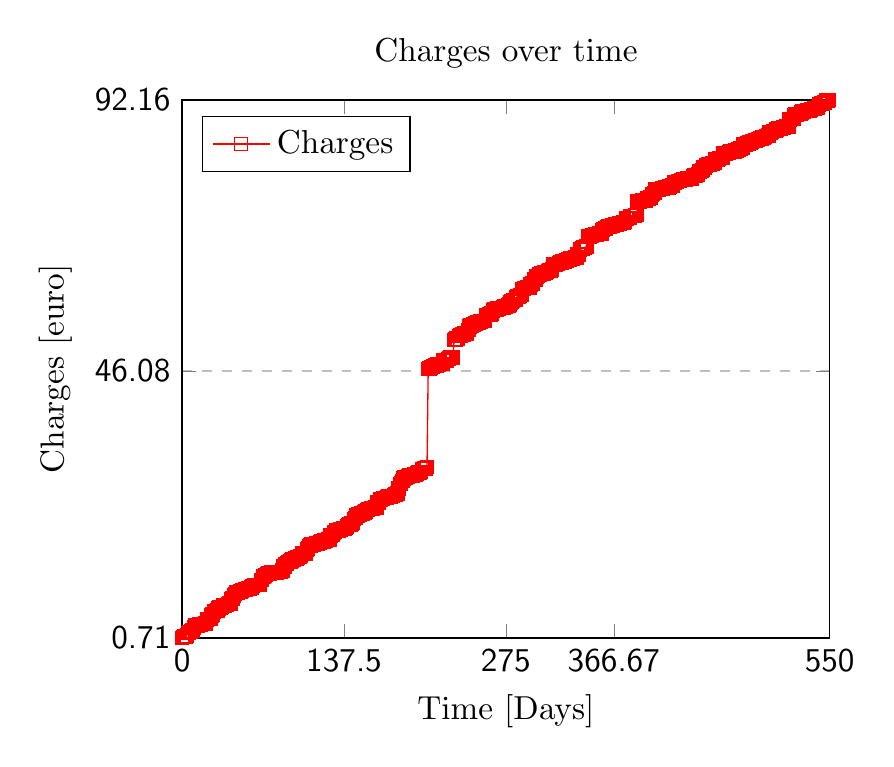
\begin{tikzpicture}[thick, scale=1.2]
\begin{axis}[
title={Charges over time},
xlabel={Time [Days]},
ylabel={Charges [euro]},
xmin=0,xmax=550,
ymin=0.713,ymax=92.162,
xtick={0,137.5,275,366.666666666667,550},
ytick={0.713,0.3565,0,46.081,92.162},
legend pos=north west,
ymajorgrids=true,
grid style=dashed,
]
\addplot[
color=red,
mark=square,
]
coordinates {
(0,0.713)(1,0.878)(2,0.94)(3,0.98)(4,1.117)(5,1.518)(6,1.637)(7,1.704)(8,1.909)(9,1.97)(10,2.523)(11,2.809)(12,2.827)(13,2.852)(14,2.887)(15,2.957)(16,3.035)(17,3.055)(18,3.069)(19,3.112)(20,3.132)(21,3.855)(22,3.939)(23,3.947)(24,3.957)(25,4.526)(26,4.684)(27,5.195)(28,5.273)(29,5.273)(30,5.347)(31,5.686)(32,5.885)(33,5.885)(34,5.965)(35,6.22)(36,6.244)(37,6.304)(38,6.313)(39,6.49)(40,6.514)(41,6.541)(42,7.312)(43,7.413)(44,7.915)(45,8.183)(46,8.437)(47,8.473)(48,8.496)(49,8.597)(50,8.649)(51,8.765)(52,8.828)(53,8.828)(54,8.913)(55,9.025)(56,9.121)(57,9.154)(58,9.22)(59,9.28)(60,9.534)(61,9.685)(62,9.707)(63,9.74)(64,9.74)(65,9.74)(66,9.74)(67,10.551)(68,10.555)(69,11.14)(70,11.238)(71,11.41)(72,11.575)(73,11.621)(74,11.647)(75,11.767)(76,11.79)(77,11.812)(78,11.82)(79,11.82)(80,11.82)(81,11.885)(82,11.899)(83,11.9)(84,11.9)(85,12.13)(86,12.814)(87,12.863)(88,13.294)(89,13.382)(90,13.621)(91,13.631)(92,13.691)(93,13.912)(94,14.056)(95,14.076)(96,14.226)(97,14.246)(98,14.404)(99,14.484)(100,14.585)(101,14.649)(102,15.044)(103,15.059)(104,15.059)(105,15.075)(106,15.783)(107,15.929)(108,16.316)(109,16.411)(110,16.559)(111,16.575)(112,16.603)(113,16.699)(114,16.799)(115,16.799)(116,16.879)(117,16.983)(118,17.064)(119,17.076)(120,17.151)(121,17.237)(122,17.255)(123,17.384)(124,17.392)(125,17.392)(126,18.167)(127,18.195)(128,18.203)(129,18.646)(130,18.714)(131,18.934)(132,18.96)(133,19.02)(134,19.164)(135,19.164)(136,19.254)(137,19.294)(138,19.302)(139,19.402)(140,19.636)(141,19.901)(142,19.947)(143,20.008)(144,20.212)(145,20.273)(146,20.946)(147,21.09)(148,21.473)(149,21.535)(150,21.646)(151,21.722)(152,21.812)(153,21.902)(154,21.964)(155,22.044)(156,22.245)(157,22.434)(158,22.521)(159,22.625)(160,22.626)(161,22.691)(162,22.742)(163,22.822)(164,22.864)(165,22.873)(166,23.75)(167,23.766)(168,24.234)(169,24.264)(170,24.344)(171,24.476)(172,24.507)(173,24.512)(174,24.618)(175,24.711)(176,24.795)(177,24.803)(178,24.825)(179,24.835)(180,24.988)(181,25.088)(182,25.164)(183,25.27)(184,26.076)(185,26.865)(186,27)(187,27.415)(188,27.824)(189,27.982)(190,28.015)(191,28.033)(192,28.154)(193,28.288)(194,28.317)(195,28.34)(196,28.356)(197,28.468)(198,28.528)(199,28.605)(200,28.757)(201,28.858)(202,28.87)(203,28.906)(204,29.394)(205,29.412)(206,29.485)(207,29.493)(208,29.749)(209,46.441)(210,46.497)(211,46.607)(212,46.738)(213,46.867)(214,46.94)(215,46.974)(216,47.002)(217,47.167)(218,47.185)(219,47.255)(220,47.266)(221,47.271)(222,47.823)(223,47.868)(224,47.885)(225,47.89)(226,48.11)(227,48.314)(228,48.334)(229,48.351)(230,48.37)(231,51.361)(232,51.439)(233,51.556)(234,51.584)(235,52.034)(236,52.1)(237,52.12)(238,52.236)(239,52.315)(240,52.455)(241,52.46)(242,52.508)(243,53.029)(244,53.692)(245,53.797)(246,53.839)(247,53.969)(248,53.982)(249,54.177)(250,54.261)(251,54.299)(252,54.306)(253,54.533)(254,54.545)(255,54.575)(256,54.586)(257,54.594)(258,55.6)(259,55.615)(260,55.63)(261,55.722)(262,55.729)(263,55.872)(264,56.413)(265,56.497)(266,56.504)(267,56.515)(268,56.716)(269,56.745)(270,56.776)(271,56.784)(272,56.81)(273,56.899)(274,57.011)(275,57.035)(276,57.126)(277,57.264)(278,57.383)(279,57.775)(280,57.94)(281,58.015)(282,58.121)(283,58.137)(284,58.653)(285,58.725)(286,58.748)(287,58.933)(288,59.013)(289,60.024)(290,60.031)(291,60.165)(292,60.17)(293,60.257)(294,60.262)(295,60.266)(296,60.831)(297,60.926)(298,60.964)(299,61.617)(300,61.623)(301,62.154)(302,62.254)(303,62.467)(304,62.537)(305,62.692)(306,62.7)(307,62.7)(308,62.835)(309,62.845)(310,62.925)(311,63.066)(312,63.124)(313,63.197)(314,63.302)(315,64.179)(316,64.207)(317,64.233)(318,64.242)(319,64.278)(320,64.468)(321,64.523)(322,64.571)(323,64.671)(324,64.713)(325,64.737)(326,64.863)(327,64.892)(328,65.025)(329,65.071)(330,65.185)(331,65.189)(332,65.219)(333,65.283)(334,65.335)(335,65.359)(336,65.875)(337,65.918)(338,66.728)(339,66.841)(340,66.868)(341,67.031)(342,67.06)(343,67.221)(344,67.261)(345,68.937)(346,68.947)(347,69.003)(348,69.075)(349,69.201)(350,69.213)(351,69.238)(352,69.25)(353,69.356)(354,69.404)(355,69.436)(356,69.444)(357,70.018)(358,70.188)(359,70.263)(360,70.322)(361,70.587)(362,70.595)(363,70.655)(364,70.71)(365,70.792)(366,70.838)(367,70.926)(368,70.933)(369,70.956)(370,71.068)(371,71.183)(372,71.189)(373,71.233)(374,71.252)(375,71.312)(376,71.433)(377,71.982)(378,72.006)(379,72.082)(380,72.113)(381,72.417)(382,72.438)(383,72.446)(384,72.454)(385,72.623)(386,72.63)(387,74.853)(388,74.864)(389,74.88)(390,74.956)(391,75.054)(392,75.061)(393,75.068)(394,75.076)(395,75.375)(396,75.428)(397,75.518)(398,75.544)(399,76.084)(400,76.184)(401,76.357)(402,76.888)(403,76.93)(404,76.939)(405,76.951)(406,77.018)(407,77.044)(408,77.134)(409,77.216)(410,77.223)(411,77.246)(412,77.278)(413,77.308)(414,77.484)(415,77.558)(416,77.581)(417,77.588)(418,78.101)(419,78.201)(420,78.212)(421,78.356)(422,78.364)(423,78.378)(424,78.554)(425,78.575)(426,78.585)(427,78.598)(428,78.622)(429,78.753)(430,78.77)(431,78.793)(432,78.797)(433,78.837)(434,79.243)(435,79.302)(436,79.341)(437,79.431)(438,79.496)(439,80.015)(440,80.022)(441,80.09)(442,80.261)(443,80.683)(444,80.708)(445,81.047)(446,81.109)(447,81.198)(448,81.233)(449,81.301)(450,81.308)(451,81.356)(452,81.435)(453,81.984)(454,82.009)(455,82.048)(456,82.16)(457,82.268)(458,82.281)(459,82.288)(460,83.013)(461,83.05)(462,83.057)(463,83.134)(464,83.137)(465,83.313)(466,83.384)(467,83.406)(468,83.414)(469,83.437)(470,83.52)(471,83.588)(472,83.696)(473,83.714)(474,83.87)(475,83.99)(476,84.006)(477,84.544)(478,84.559)(479,84.628)(480,84.784)(481,84.791)(482,84.917)(483,84.947)(484,85.14)(485,85.164)(486,85.179)(487,85.286)(488,85.375)(489,85.472)(490,85.523)(491,85.583)(492,85.587)(493,85.796)(494,85.811)(495,85.844)(496,86.006)(497,86.031)(498,86.1)(499,86.609)(500,86.638)(501,86.706)(502,86.858)(503,86.884)(504,86.906)(505,87.088)(506,87.335)(507,87.343)(508,87.354)(509,87.383)(510,87.41)(511,87.473)(512,87.578)(513,87.6)(514,87.625)(515,87.638)(516,88.826)(517,88.932)(518,88.936)(519,88.947)(520,89.629)(521,89.637)(522,89.722)(523,89.746)(524,89.775)(525,89.797)(526,89.99)(527,90.235)(528,90.242)(529,90.251)(530,90.26)(531,90.325)(532,90.37)(533,90.405)(534,90.536)(535,90.585)(536,90.612)(537,90.749)(538,90.785)(539,90.812)(540,90.859)(541,91.388)(542,91.434)(543,91.556)(544,91.576)(545,91.746)(546,91.753)(547,92.035)(548,92.067)(549,92.162)
};
\legend{Charges}
\end{axis}
\end{tikzpicture}


%\subsubsection{Charges plot}
%Removed to preserve my eyes from the colors....!!!!\\
%\includegraphics[scale=0.3]{Charges2.png}

\subsubsection{Charges kiviat}
%One note :-) This should be random! Maybe not...
\input{chargesKiviat}

%\subsubsection{Table}
%\begin{longtable}{|c|c|c|c|c|}
\hline
\multicolumn{5}{|c|}{Cashflows} \\
\hline
Category & Debit & Credit & PnL \\
\hline
Cmb & 6866 & -963 & -7829\\
\hline
Debt & 25532 & 0 & -25532\\
\hline
Food & 19400 & 0 & -19400\\
\hline
Swap & 16683 & 0 & -16683\\
\hline
Other & 13685 & 0 & -13685\\
\hline
Toxics & 13497 & 0 & -13497\\
\hline
Cash & 12936 & 0 & -12936\\
\hline
Bank & 6625 & 0 & -6625\\
\hline
Rent & 5785 & 0 & -5785\\
\hline
Taxes & 4177 & 0 & -4177\\
\hline
Port & 3481 & 0 & -3481\\
\hline
Funding & 2700 & 0 & -2700\\
\hline
Telephone & 2357 & 0 & -2357\\
\hline
Health & 1505 & 0 & -1505\\
\hline
Investments & 1188 & 0 & -1188\\
\hline
Transport & 1166 & 0 & -1166\\
\hline
Car & 988 & 0 & -988\\
\hline
Energy & 568 & 0 & -568\\
\hline
Home & 519 & 0 & -519\\
\hline
Boat & 408 & 0 & -408\\
\hline
Crooks & 249 & 0 & -249\\
\hline
Presents & 105 & 0 & -105\\
\hline
 ... & ... & ... & ...\\
\hline
 Total & 140420 & 142872 & 2452 \\
\hline
\end{longtable}


\subsubsection{Histogram of the charges}
\begin{bchart}[min=0,max=25,step=5,unit=k\texteuro]
\bcbar[label=Cmb]{6}\\
\smallskip
\bcbar[label=Debt]{25}\\
\smallskip
\bcbar[label=Food]{19}\\
\smallskip
\bcbar[label=Swap]{16}\\
\smallskip
\bcbar[label=Other]{13}\\
\smallskip
\bcbar[label=Toxics]{13}\\
\smallskip
\bcbar[label=Cash]{12}\\
\smallskip
\bcbar[label=Bank]{6}\\
\smallskip
\bcbar[label=Rent]{5}\\
\smallskip
\bcbar[label=Taxes]{4}\\
\smallskip
\bcbar[label=Port]{3}\\
\smallskip
\bcbar[label=Funding]{2}\\
\smallskip
\bcbar[label=Telephone]{2}\\
\smallskip
\bcbar[label=Health]{1}\\
\smallskip
\bcbar[label=Investments]{1}\\
\smallskip
\bcbar[label=Transport]{1}\\
\smallskip
\bcbar[label=Car]{0}\\
\smallskip
\bcbar[label=Energy]{0}\\
\smallskip
\bcbar[label=Home]{0}\\
\smallskip
\bcbar[label=Boat]{0}\\
\smallskip
\bcbar[label=Crooks]{0}\\
\smallskip
\bcbar[label=Presents]{0}\\
\smallskip
\end{bchart}


%\subsubsection{Chart}

%\subsubsection{Cheese}
%\begin{tikzpicture}[scale=2]
\foreach \p/\t in {
4 / Cmb-6.866k\texteuro ,
18 / Debt-25.532k\texteuro ,
13 / Food-19.4k\texteuro ,
11 / Swap-16.683k\texteuro ,
9 / Other-13.685k\texteuro ,
9 / Toxics-13.497k\texteuro ,
9 / Cash-12.936k\texteuro ,
4 / Bank-6.625k\texteuro ,
4 / Rent-5.785k\texteuro ,
2 / Taxes-4.177k\texteuro ,
2 / Port-3.481k\texteuro ,
1 / Funding-2.7k\texteuro ,
1 / Telephone-2.357k\texteuro ,
1 / Health-1.505k\texteuro ,
0 / Investments-1.188k\texteuro ,
0 / Transport-1.166k\texteuro ,
0 / Car-0.988k\texteuro ,
0 / Energy-0.568k\texteuro ,
0 / Home-0.519k\texteuro ,
0 / Boat-0.408k\texteuro ,
0 / Crooks-0.249k\texteuro ,
0 / Presents-0.105k\texteuro ,
}
  {
\setcounter{a}{\value{b}}
\addtocounter{b}{\p}
\slice{\thea/100*360}
          {\theb/100*360}
          {\p\%}{\t}
  }
\end{tikzpicture}


\subsection{Incomes}
%Data are aggregated between Initial date: \textbf{2000-01-01} and Last date: \textbf{2018-11-16 00:00:00}


%\subsubsection{Table}
%\begin{longtable}{|c|c|c|c|c|}
\hline
\multicolumn{5}{|c|}{Cashflows} \\
\hline
Category & Debit & Credit & PnL \\
\hline
Salary & 0 & 86580 & 86580\\
\hline
Funding & 0 & 42600 & 42600\\
\hline
Cmb & 0 & 7287 & 7287\\
\hline
Bank & 0 & 6097 & 6097\\
\hline
Debt & 0 & 2549 & 2549\\
\hline
Taxes & 0 & 1824 & 1824\\
\hline
Other & 0 & 1191 & 1191\\
\hline
Rent & 0 & 149 & 149\\
\hline
Telephone & 0 & 128 & 128\\
\hline
 ... & ... & ...\\
\hline
 Total & 140420 & 142872 & 2452 \\
\hline
\end{longtable}

\subsubsection{Histogram}
\begin{bchart}[min=0,max=86,step=17,unit=k\texteuro]
\bcbar[label=Salary]{86}\\
\smallskip
\bcbar[label=Funding]{42}\\
\smallskip
\bcbar[label=Cmb]{7}\\
\smallskip
\bcbar[label=Bank]{6}\\
\smallskip
\bcbar[label=Debt]{2}\\
\smallskip
\bcbar[label=Taxes]{1}\\
\smallskip
\bcbar[label=Other]{1}\\
\smallskip
\bcbar[label=Rent]{0}\\
\smallskip
\bcbar[label=Telephone]{0}\\
\smallskip
\end{bchart}

\subsubsection{Curve}
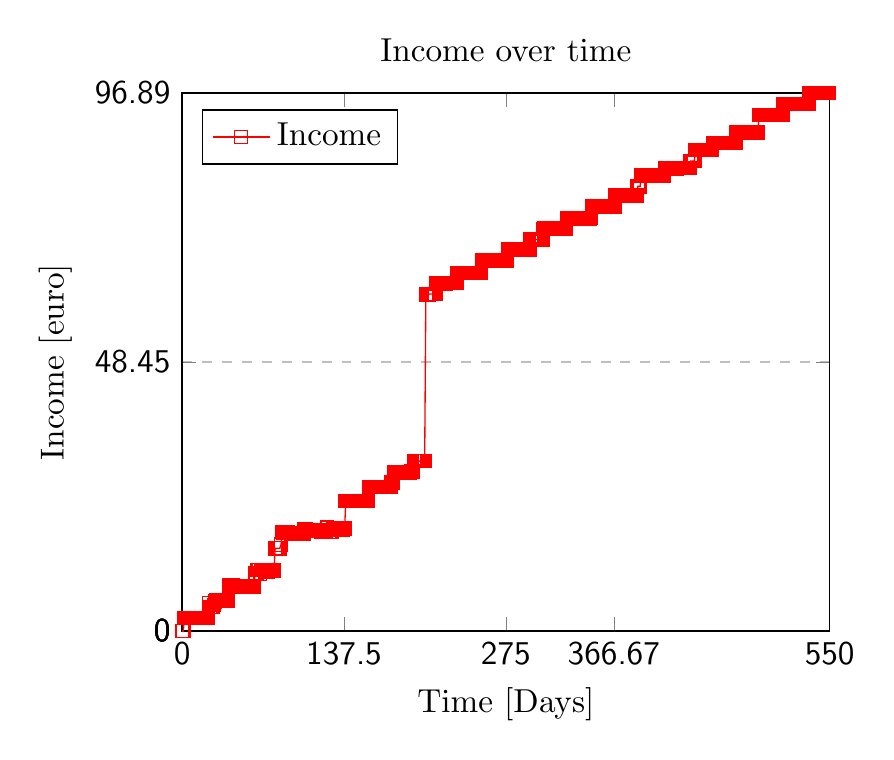
\begin{tikzpicture}[thick, scale=1.2]
\begin{axis}[
title={Income over time},
xlabel={Time [Days]},
ylabel={Income [euro]},
xmin=0,xmax=550,
ymin=0,ymax=96.89,
xtick={0,137.5,275,366.666666666667,550},
ytick={0,0,0,48.445,96.89},
legend pos=north west,
ymajorgrids=true,
grid style=dashed,
]
\addplot[
color=red,
mark=square,
]
coordinates {
(0,0)(1,0)(2,2.34)(3,2.34)(4,2.34)(5,2.34)(6,2.34)(7,2.34)(8,2.34)(9,2.34)(10,2.34)(11,2.34)(12,2.34)(13,2.34)(14,2.34)(15,2.34)(16,2.34)(17,2.34)(18,2.34)(19,2.34)(20,2.34)(21,2.34)(22,2.34)(23,5.015)(24,4.345)(25,4.345)(26,4.345)(27,4.68)(28,5.38)(29,5.485)(30,5.485)(31,5.485)(32,5.485)(33,5.485)(34,5.485)(35,5.485)(36,5.485)(37,5.485)(38,5.485)(39,5.485)(40,8.248)(41,8.248)(42,8.228)(43,8.228)(44,8.102)(45,8.112)(46,8.112)(47,8.112)(48,8.112)(49,8.002)(50,8.01)(51,8.026)(52,8.034)(53,8.034)(54,7.925)(55,7.941)(56,7.957)(57,7.965)(58,7.981)(59,7.981)(60,7.981)(61,8.005)(62,10.345)(63,10.345)(64,10.995)(65,10.995)(66,10.325)(67,10.975)(68,10.975)(69,10.975)(70,10.975)(71,10.724)(72,10.621)(73,10.713)(74,10.803)(75,10.865)(76,10.865)(77,10.881)(78,10.889)(79,14.889)(80,14.899)(81,14.91)(82,14.91)(83,14.916)(84,15.566)(85,17.83)(86,17.81)(87,17.81)(88,17.81)(89,17.81)(90,17.81)(91,17.7)(92,17.7)(93,17.596)(94,17.596)(95,17.596)(96,17.596)(97,17.596)(98,17.596)(99,17.596)(100,17.596)(101,17.596)(102,17.596)(103,17.596)(104,18.246)(105,18.246)(106,18.226)(107,18.226)(108,18.226)(109,18.226)(110,18.116)(111,18.116)(112,18.116)(113,18.116)(114,18.116)(115,18.116)(116,18.116)(117,18.116)(118,17.99)(119,17.99)(120,17.99)(121,17.99)(122,17.99)(123,18.64)(124,18.497)(125,17.827)(126,17.827)(127,17.827)(128,18.477)(129,18.477)(130,18.477)(131,18.264)(132,18.28)(133,18.28)(134,18.288)(135,18.334)(136,18.342)(137,18.44)(138,18.448)(139,23.448)(140,23.448)(141,23.448)(142,23.448)(143,23.448)(144,23.448)(145,23.448)(146,23.448)(147,23.448)(148,23.448)(149,23.448)(150,23.448)(151,23.448)(152,23.448)(153,23.448)(154,23.448)(155,23.448)(156,23.448)(157,23.448)(158,23.448)(159,25.937)(160,25.937)(161,25.937)(162,25.937)(163,25.937)(164,25.937)(165,25.937)(166,25.937)(167,25.937)(168,25.937)(169,25.937)(170,25.937)(171,25.937)(172,25.937)(173,25.937)(174,25.937)(175,25.937)(176,25.937)(177,25.937)(178,26.737)(179,26.737)(180,28.562)(181,28.562)(182,28.562)(183,28.562)(184,28.562)(185,28.562)(186,28.562)(187,28.562)(188,28.562)(189,28.562)(190,28.562)(191,28.562)(192,28.562)(193,28.565)(194,28.685)(195,28.693)(196,28.709)(197,30.605)(198,30.605)(199,30.605)(200,30.605)(201,30.605)(202,30.605)(203,30.605)(204,30.605)(205,30.605)(206,30.605)(207,60.605)(208,60.605)(209,60.605)(210,60.704)(211,60.704)(212,60.704)(213,60.704)(214,60.704)(215,60.704)(216,62.595)(217,62.6)(218,62.6)(219,62.6)(220,62.6)(221,62.6)(222,62.6)(223,62.6)(224,62.6)(225,62.704)(226,62.704)(227,62.704)(228,62.704)(229,62.704)(230,62.704)(231,62.704)(232,62.704)(233,62.704)(234,64.462)(235,64.462)(236,64.462)(237,64.462)(238,64.462)(239,64.462)(240,64.462)(241,64.462)(242,64.462)(243,64.462)(244,64.462)(245,64.462)(246,64.462)(247,64.462)(248,64.462)(249,64.462)(250,64.462)(251,64.462)(252,64.462)(253,64.462)(254,64.462)(255,66.774)(256,66.774)(257,66.774)(258,66.774)(259,66.774)(260,66.774)(261,66.774)(262,66.774)(263,66.774)(264,66.774)(265,66.774)(266,66.774)(267,66.774)(268,66.774)(269,66.774)(270,66.774)(271,66.774)(272,66.774)(273,66.774)(274,66.774)(275,66.787)(276,66.787)(277,68.729)(278,68.729)(279,68.729)(280,68.729)(281,68.729)(282,68.729)(283,68.729)(284,68.729)(285,68.729)(286,68.729)(287,68.729)(288,68.729)(289,68.729)(290,68.729)(291,68.729)(292,68.729)(293,68.729)(294,68.729)(295,68.729)(296,70.516)(297,70.516)(298,70.516)(299,70.516)(300,70.516)(301,70.516)(302,70.516)(303,70.516)(304,70.516)(305,70.516)(306,70.516)(307,72.443)(308,72.468)(309,72.468)(310,72.468)(311,72.468)(312,72.488)(313,72.488)(314,72.488)(315,72.488)(316,72.488)(317,72.488)(318,72.488)(319,72.488)(320,72.488)(321,72.488)(322,72.488)(323,72.488)(324,72.488)(325,72.488)(326,72.488)(327,74.347)(328,74.347)(329,74.347)(330,74.347)(331,74.347)(332,74.347)(333,74.347)(334,74.347)(335,74.347)(336,74.347)(337,74.347)(338,74.347)(339,74.347)(340,74.347)(341,74.347)(342,74.347)(343,74.347)(344,74.347)(345,74.347)(346,74.347)(347,74.359)(348,76.486)(349,76.486)(350,76.486)(351,76.486)(352,76.486)(353,76.486)(354,76.486)(355,76.486)(356,76.486)(357,76.486)(358,76.486)(359,76.486)(360,76.486)(361,76.486)(362,76.486)(363,76.486)(364,76.486)(365,76.486)(366,76.486)(367,76.486)(368,78.405)(369,78.42)(370,78.42)(371,78.42)(372,78.42)(373,78.42)(374,78.42)(375,78.42)(376,78.42)(377,78.42)(378,78.42)(379,78.42)(380,78.42)(381,78.42)(382,78.42)(383,78.42)(384,78.42)(385,78.42)(386,78.42)(387,80.09)(388,80.09)(389,80.09)(390,82.027)(391,82.027)(392,82.027)(393,82.027)(394,82.027)(395,82.027)(396,82.027)(397,82.027)(398,82.027)(399,82.027)(400,82.027)(401,82.027)(402,82.027)(403,82.027)(404,82.027)(405,82.027)(406,82.027)(407,82.027)(408,82.027)(409,82.027)(410,83.303)(411,83.303)(412,83.303)(413,83.303)(414,83.303)(415,83.303)(416,83.303)(417,83.303)(418,83.303)(419,83.303)(420,83.303)(421,83.38)(422,83.38)(423,83.38)(424,83.38)(425,83.38)(426,83.38)(427,83.38)(428,83.38)(429,83.38)(430,83.38)(431,83.38)(432,84.631)(433,84.631)(434,84.631)(435,84.631)(436,86.631)(437,86.631)(438,86.631)(439,86.631)(440,86.631)(441,86.631)(442,86.631)(443,86.631)(444,86.631)(445,86.631)(446,86.631)(447,86.631)(448,86.631)(449,86.631)(450,86.631)(451,87.888)(452,87.888)(453,87.888)(454,87.888)(455,87.888)(456,87.888)(457,87.888)(458,87.888)(459,87.888)(460,87.888)(461,87.888)(462,87.888)(463,87.888)(464,87.888)(465,87.888)(466,87.888)(467,87.888)(468,87.888)(469,87.888)(470,87.888)(471,89.814)(472,89.814)(473,89.814)(474,89.814)(475,89.814)(476,89.814)(477,89.814)(478,89.814)(479,89.814)(480,89.814)(481,89.814)(482,89.814)(483,89.814)(484,89.814)(485,89.814)(486,89.814)(487,89.814)(488,89.814)(489,89.814)(490,92.943)(491,92.943)(492,92.958)(493,92.958)(494,92.958)(495,92.958)(496,92.958)(497,92.958)(498,92.958)(499,92.958)(500,92.958)(501,92.958)(502,92.958)(503,92.958)(504,92.958)(505,92.958)(506,92.958)(507,92.958)(508,92.958)(509,92.958)(510,92.958)(511,94.89)(512,94.89)(513,94.89)(514,94.89)(515,94.89)(516,94.89)(517,94.89)(518,94.89)(519,94.89)(520,94.89)(521,94.89)(522,94.89)(523,94.89)(524,94.89)(525,94.89)(526,94.89)(527,94.89)(528,94.89)(529,94.89)(530,94.89)(531,94.89)(532,94.89)(533,96.89)(534,96.89)(535,96.89)(536,96.89)(537,96.89)(538,96.89)(539,96.89)(540,96.89)(541,96.89)(542,96.89)(543,96.89)(544,96.89)(545,96.89)(546,96.89)(547,96.89)(548,96.89)(549,96.89)
};
\legend{Income}
\end{axis}
\end{tikzpicture}

%\includegraphics[width=.8\textwidth]{Income.png}


%%%%%%%%%%%%%%%%%%%%%%%%%%%%%%%%%%%%%%%%%%%%%%%%%%%%%%%%%%%%%%%%%%%%%%%%%%%%%%%%%%%%%%%%%%%%%%%%%%%%%%%%%%%%%%%%%%%%%%%%%%%%%%%%%%%%%%%%%%%%%%%%%%%%%%%%%%%%%%

\end{document}

